\documentclass[a4paper]{article}
\usepackage[pdftex]{graphicx}
\usepackage[utf8]{inputenc}
\usepackage{enumerate}
\usepackage{siunitx}
\sisetup{locale=DE}
\DeclareSIUnit \massunit {u}
\usepackage{icomma}
\usepackage{amssymb}
\hyphenation{Ver-simplification}
\usepackage{tikz}
\usepackage{href-ul}
\hypersetup{
	colorlinks=true,
	linkcolor=blue,
	urlcolor=blue}
\usepackage{geometry}
\geometry{a4paper, top=15mm, left=15mm, right=15mm, bottom=15mm,
	headsep=10mm, footskip=12mm}

\begin{document}
	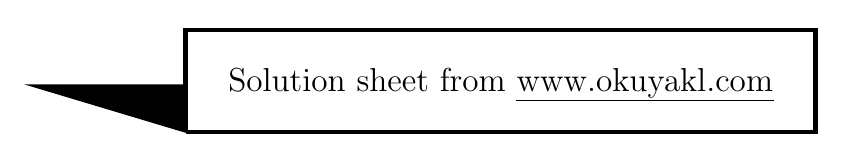
\begin{tikzpicture}(10,3)
		\draw[ultra thick](2,0) --(10,0) -- (10,1.3) --(2,1.3) -- (2,0);
		\draw[fill=black](2,0)-- (0,.6) -- (2,.6) -- (2,0);
		\node at (6,.6) {\large Solution sheet from \href{http://www.okuyakl.com}{www.okuyakl.com}};
	\end{tikzpicture}
	\vspace{0.5 cm}
	
	
	\noindent{\bf Task 1.}\\
	The sum of the individual impulses, the total impulse, is the same before and after the collision. It doesn't matter whether the impact is elastic or inelastic.
	\vspace{0.5 cm}
	
	\noindent{\bf Task 2. a)}\\
	The following relationship applies to the inelastic collision. Here $v_1$ and $m_1$ are the speed in $\SI{}{\meter\over\second}$ and the mass of the minibus, $v_2$ and $m_2$ are the speed and mass of the small car. After the impact, both vehicles continue to move together at the same speed $u$:
	
	$$
	\renewcommand{\arraystretch}{2}
	\begin{array}{rcll}
		m_1 v_1 + m_2 v_2 &=&(m_1 + m_2)\cdot u &|:(m_1 + m_2) \\
		u &=& {m_1 v_1 + m_2 v_2 \over m_1 + m_2} \\
		u &=& {\SI{1700}{\kilogram} \cdot \SI{15}{\meter\over\second} + \SI{650}{\kilogram} \cdot (\SI{-10}{\ meter\over\second})\over \SI{1700}{\kilogram} + \SI{650}{\kilogram}} & = \SI{8,1}{\meter\over\second}
	\end{array}
	$$
	$u$ has the same sign as $v_1~\Rightarrow$ Both vehicles move with $u=\SI{8,1}{\meter\over\second} = \SI{29}{\kilo\meter\over \hour}$ continue in the direction of travel of the minibus.
	\vspace{0.5 cm}
	
	\noindent{\bf Task 2. b)}\\
	We compare the total energy before the collision $E_{kin,v}$ with that after the collision $E_{kin,n}$. The kinetic energy after an elastic collision decreases. The difference is converted into deformation work and internal energy $E_{v,i}$.
	$$
	\renewcommand{\arraystretch}{2}
	\begin{array}{rcl}
		E_{v,i} & = & \Delta E_{kin} = E_{kin,v} - E_{kin,n} \\
		& = & {1 \over 2}m_1 \cdot v_1^2 + {1 \over 2}m_2 \cdot v_2^2
		- {1 \over 2}\cdot (m_1+m_2) \cdot u^2 \\
		& = & {1 \over 2}\cdot \SI{1700}{\kilogram} \cdot (\SI{15}{\meter\over\second})^2 + {1 \over 2}\cdot\SI {650}{\kilogram} \cdot (\SI{10}{\meter\over\second})^2
		- {1 \over 2}\cdot (\SI{1700}{\kilogram} + \SI{650}{\kilogram}) \cdot (\SI{8,1}{\meter\over\second})^ 2\\
		& = & \SI{223750}{\joule} - \SI{77092}{\joule}\\
		& = & \SI{146658}{\joule} \approx \SI{150}{\kilo\joule}
	\end{array}
	$$
	The percentage $x \%$ of the deformation work of the total energy is:
	$$ x\% = {E_{v,i}\over E_{kin,v}}\cdot 100\%= 66\%$$
	\vspace{0.5 cm}
	
	\noindent{\bf Task 3. a)}\\
	Force $F$ is equal to change in momentum $\Delta p $ with time:
	$$F = {\Delta p \over \Delta t} \qquad (*) $$
	Momentum equals mass times velocity; Here the mass of the rocket changes, the speed of the combustion gases remains constant, so the change in momentum here is equal to the change in mass $\Delta m$ in the time interval $ \Delta t = \SI{1}{\second}$ times the speed. $(*)$ then becomes:
	$$F= {\Delta m \cdot v \over \Delta t} \Leftrightarrow {\Delta m \over \Delta t}= {F \over v}$$
	$$ {\Delta m \over \Delta t} = {\SI{2.0e5}{\newton} \over \SI{2000}{\meter\over\second}} = \SI{100}{kg \over s}$$
	Unit check:
	$$ {\SI{}{\newton\over{\meter\over\second}}}= \SI{}{\kilogram\cdot {\meter\over{\second^2}} \over {\meter\over\ second}} = \SI{}{\kilogram\over \second}$$
	$\SI{100}{\kilogram}$ fuel had to be burned per second.
	\vspace{0.5 cm}
	
	\noindent{\bf Task 3. b)}\\
	The accelerating force is equal to the difference between the thrust force and the weight force. According to the law of inertia we get $a$ for the acceleration:
	$$
	\renewcommand{\arraystretch}{2}
	\begin{array}{rcll}
		F_a &=& F_{thrust}-F_G &\stackrel{!}{=} m \cdot a\\
		a &=& {F_{thrust}-F_G \over m} & = {\SI{2.0e5}{\newton} - \SI{10000}{\kilogram}\cdot \SI{9.81}{\ meter\over{\second^2}} \over \SI{10000}{\kilogram} }\\
		a &=& \SI{10}{\meter \over {\second^2}}
	\end{array}
	$$
	\vspace{0.5 cm}
	
	\noindent{\bf Task 4. a)}\\
	Impulse before decay = impulse after decay:
	$$
	\renewcommand{\arraystretch}{2}
	\begin{array}{rcll}
		0 &=& m_1v_1 + m_2v_2 \\
		v_1 &=& - {m_2 \over m_1}v_2 \\
		v_1 &=& -{\SI{4}{\massunit} \over \SI{234}{\massunit}} \cdot\SI{1,4e7}{\meter\over \second}\\
		v_1 &=& \SI{-2,4e5}{\meter\over \second}
	\end{array}
	$$
	\vspace{0.5 cm}
	
	\noindent{\bf Task 4. b)}\\
	The ratio of both kinetic energies can be calculated without precisely determining them individually:
	$$
	{E_{kin1}\over E_{kin2}}= {{1 \over 2}m_1v_1^2 \over {1 \over 2} m_2v_2^2} = { \SI{234}{\massunit} \cdot (\SI{2,4e5}{\meter\over \second})^2 \over \SI{4}{\massunit}\cdot (\SI {1.4e7}{\meter\over\second})^2}=0.0172 \approx 1 : 58$$
	\vspace{0.5 cm}
	
	\noindent{\bf Task 5.}\\
	The asteroid's momentum was:
	$$p=m_1v_1=\SI{7,0e13}{\kilogram} \cdot \SI{20e3}{\meter\over \second} = \SI{1,4e18}{\newton\cdot\second}$$
	This gives the earth a change in speed of:
	$$
	\renewcommand{\arraystretch}{2}
	\begin{array}{rcll}
		m_1v_1 &=& (m_1+m_2)u \\
		u &=& {m_1v_1 \over m_1+m_2}\\
		u &=& {\SI{1.4e18}{\newton\cdot\second}\over\SI{5.97e24}{\kilogram} +\SI{7.0e13}{\kilogram}}\\
		u &=& \SI{2,3e-7}{\meter\over \second}
	\end{array}
	$$
	The speed after the impact is minimal and the Earth remains in its orbit.
	(Orbital speed of the Earth relative to the Sun: $v \approx \SI{30}{\kilo\meter\over \second}$)
	\vspace{0.5 cm}
	
	\noindent{\bf Task 6. a)}\\
	The velocity of the mass $m_2$ before momentum transfer is:
	$$v_2 = \sqrt{2gh} = \sqrt{2\cdot \SI{9.81}{\meter \over {\second^2}} \cdot \SI{0.30}{\meter}}=\SI {2,4}{\meter\over \second}$$
	The mass $m_1$ then gets the speed:
	$$
	\renewcommand{\arraystretch}{2}
	\begin{array}{rcll}
		m_2v_2 &=& (m_1+m_2)u \\
		u &=& {m_2v_2 \over m_1 + m_2} \\
		u &=& \SI{1,1}{\meter\over\second}
	\end{array}
	$$
	\vspace{0.5 cm}
	
	\noindent{\bf Task 6. b)}\\
	The potential energy gained as the mass $m_1$ rises is:
	$$E_{pot}=E_{pot1}-E_{pot2} = (m_1-m_2)gh$$
	\vspace{0.5 cm}
	
	\noindent
	\begin{minipage}{0.5\textwidth}
		We equate the kinetic energy of the system to:
		$$
		\renewcommand{\arraystretch}{2}
		\begin{array}{rcll}
			E_{pot}&=&E_{kin} \\
			(m_1-m_2)gh &=& {1 \over 2}(m_1+m_2)u^2 \\
			h &=& {(m_1 +m_2)u^2 \over 2 (m_1-m_2)g} \\
			h &=& \SI{0.56}{\meter}
		\end{array}
		$$
	\end{minipage}
	\hfill
	\begin{minipage}{0.5\textwidth}
		\begin{center}
			\includegraphics[width=7 cm]{../../viecher/eendcomic.pdf}
			
			Here you can go back to the \href{https://www.okuyakl.de/phys/p10impL136/ae136.pdf}{task sheet}
		\end{center}
		
	\end{minipage}
	
	
	%End
	\end{document}